Es wird  in  Detail  beschrieben,  welche  elektronische Komponenten aus welchem
Grund ausgew\"ahlt wurden.

% **************************************************************************** %
\subsection{36V Netzteil}
% **************************************************************************** %



% **************************************************************************** %
\subsection{LT3741}
% **************************************************************************** %

Die  Ausgangsspannung   muss   mindestens   im  Bereich  von  \SI{0}{\volt}  bis
\SI{24}{\volt}  liegen  und   einen  Rippel  kleiner  als  \SI{300}{\milli\volt}
besitzen.  Der  Ausgangsstrom muss mindestens im Bereich von \SI{0}{\ampere} bis
\SI{3.5}{\ampere} liegen  und  einen  Rippel kleiner als \SI{100}{\milli\ampere}
besitzen. Dabei  sollte  die Effizienz bei Volllast mindestens \SI{80}{\percent}
betragen.

Da  das  Endprodukt  schlussendlich  in  Serie  mit  mehreren   Spannungs-  oder
Stromquellen  geschalten  werden  k\"onnte, muss  zus\"atzlich  darauf  geachtet
werden,  dass  der Spannungswandler \emph{leistungsaufnahmef\"ahig}  sein  muss.
Diese Eigenschaft weist  ein  sogenannter  \emph{Synchronwandler}  vor und wurde
zusammen mit den Spannungs-,  Strom-,  und Leistungsanforderungen als prim\"ares
Merkmal f\"ur die Produktsuche eines Wandlers verwendet.



\begin{figure}[H]
    \center
    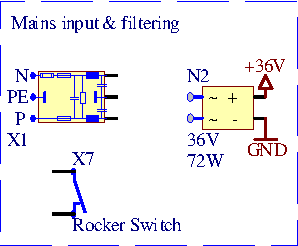
\includegraphics[width=.35\textwidth]{images/circuit/mains-input.pdf}
    \caption{Netzspannung wird gefiltert und auf 36V DC transformiert}
    \label{fig:circuit:mains-input}
\end{figure}

\begin{figure}[H]
    \center
    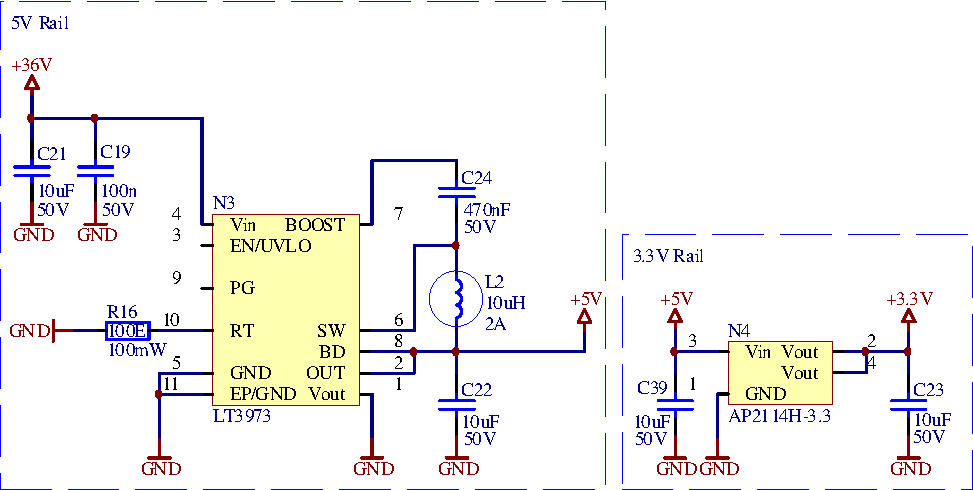
\includegraphics[width=.75\textwidth]{images/circuit/5v-3v-rails.pdf}
    \caption{Speisung f\"ur 5V mittels Abwertswandler (links) und Speisung f\"ur 3.3V mittels Linearregler (rechts)}
    \label{fig:circuit:rails}
\end{figure}

\begin{figure}[H]
    \center
    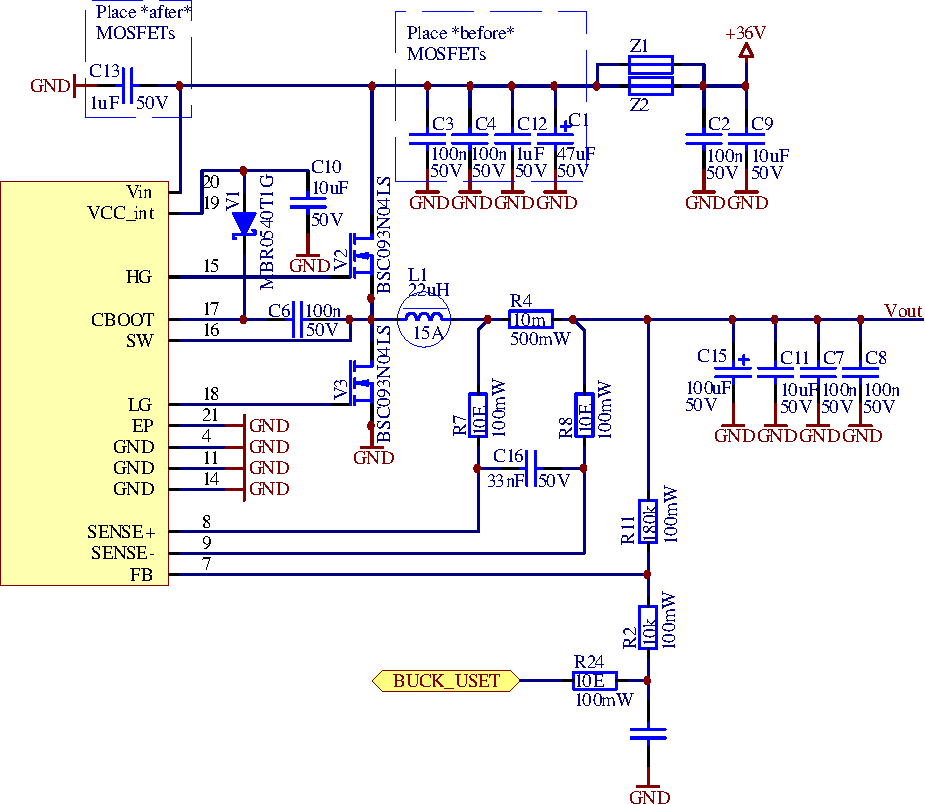
\includegraphics[width=.75\textwidth]{images/circuit/buck.pdf}
    \caption{Herzst\"uck des Projektes: Aufbau des LT3741 CVCC Synchronwandler}
    \label{fig:circuit:buck}
\end{figure}

\begin{figure}[H]
    \center
    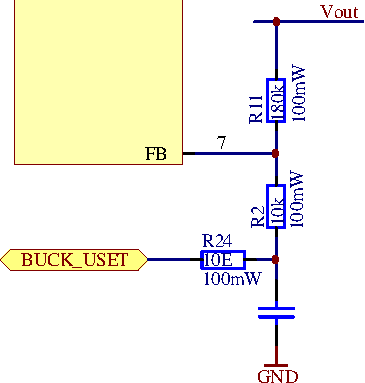
\includegraphics[width=.35\textwidth]{images/circuit/buck-uset.pdf}
    \caption{Einstellung der Ausgangsspannung durch \"Anderung der Bezugsspannung im Feedback-Loop mittels einer analogen Steuerspannung von 0V bis 1.5V}
    \label{fig:circuit:buck:uset}
\end{figure}

\begin{figure}[H]
    \center
    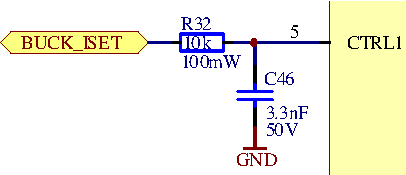
\includegraphics[width=.4\textwidth]{images/circuit/buck-iset.pdf}
    \caption{Einstellung des Maximalstroms mittels einer analogen Steuerspannung von 0V bis 1.5V}
    \label{fig:circuit:buck:iset}
\end{figure}

\begin{figure}[H]
    \center
    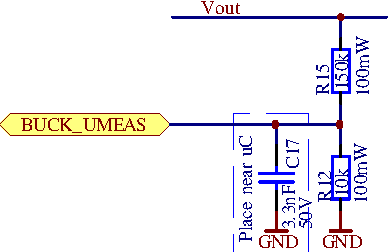
\includegraphics[width=.45\textwidth]{images/circuit/buck-umeas.pdf}
    \caption{Messen der Ausgangsspannung}
    \label{fig:circuit:buck:umeas}
\end{figure}

\begin{figure}[H]
    \center
    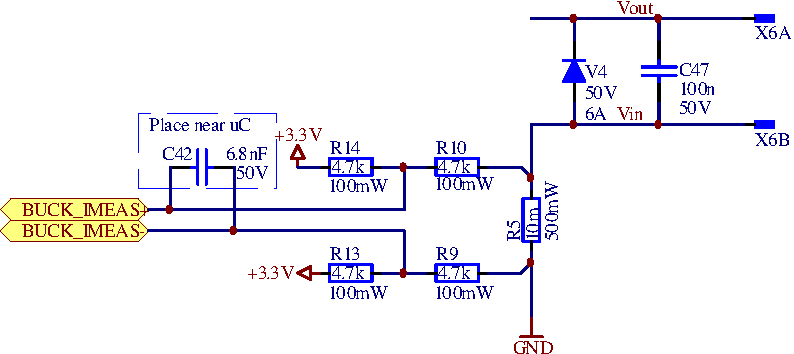
\includegraphics[width=.85\textwidth]{images/circuit/buck-imeas.pdf}
    \caption{Messen des Ausgangsstromes}
    \label{fig:circuit:buck:imeas}
\end{figure}

\begin{figure}[H]
    \center
    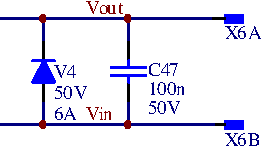
\includegraphics[width=.35\textwidth]{images/circuit/output-connectors.pdf}
    \caption{Verpolungsschutz am Ausgang}
    \label{fig:circuit:output}
\end{figure}

\begin{figure}[H]
    \center
    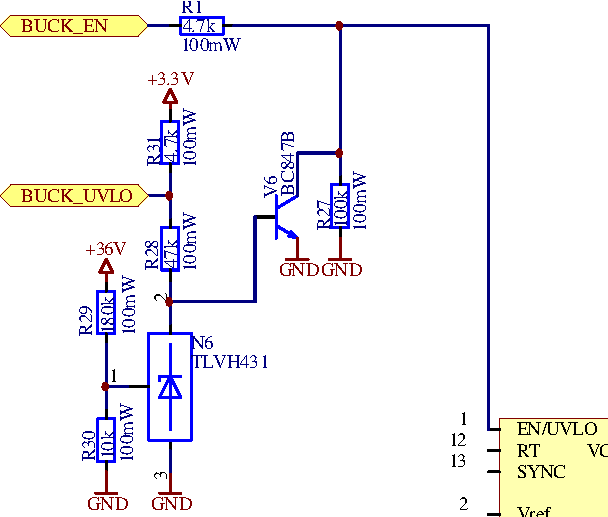
\includegraphics[width=.6\textwidth]{images/circuit/uvlo.pdf}
    \caption{Under-Voltage Lock-Out (UVLO) erm\"oglicht ein kontrolliertes Ein- und Ausschalten des Reglers}
    \label{fig:circuit:uvlo}
\end{figure}

\begin{figure}[H]
    \center
    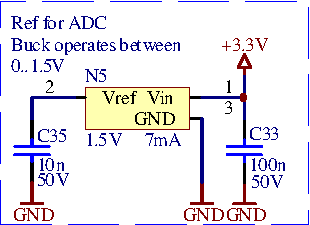
\includegraphics[width=.4\textwidth]{images/circuit/vref.pdf}
    \caption{1.5V Referenzspannung um die ADCs m\"oglichst in Full-Range betreiben zu k\"onnen}
    \label{fig:circuit:vref}
\end{figure}

\begin{figure}[H]
    \center
    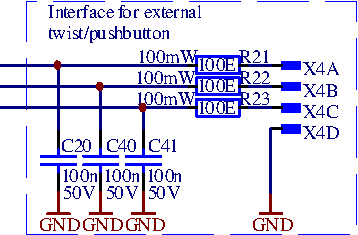
\includegraphics[width=.4\textwidth]{images/circuit/pushbutton.pdf}
    \caption{Drehdruckknopf}
    \label{fig:circuit:pushbutton}
\end{figure}

